\documentclass{article}

\usepackage{graphicx}
% \usepackage{cleveref}

\newcommand{\beginsupplement}{%
        \setcounter{table}{0}
        \renewcommand{\thetable}{S\arabic{table}}%
        \setcounter{figure}{0}
        \renewcommand{\thefigure}{S\arabic{figure}}%
     }

\begin{document}
\beginsupplement

\begin{figure*}
    \centering
    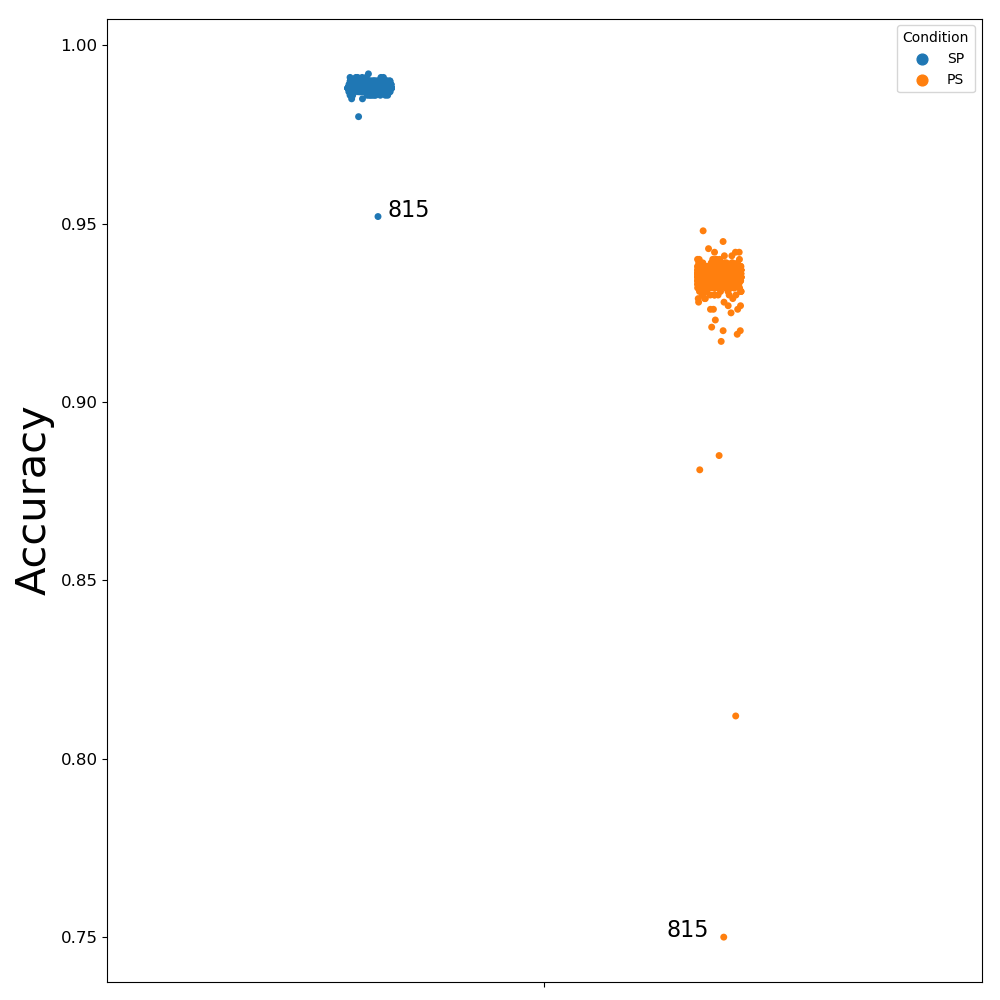
\includegraphics[width=10cm]{figures/Ablation_results_K_model.png}
    \caption{\textbf{Ablation results for the model from Gulordave et. al, 2018}}
    \label{fig:ablation_all_models}
\end{figure*}

\begin{figure*}
    \centering
    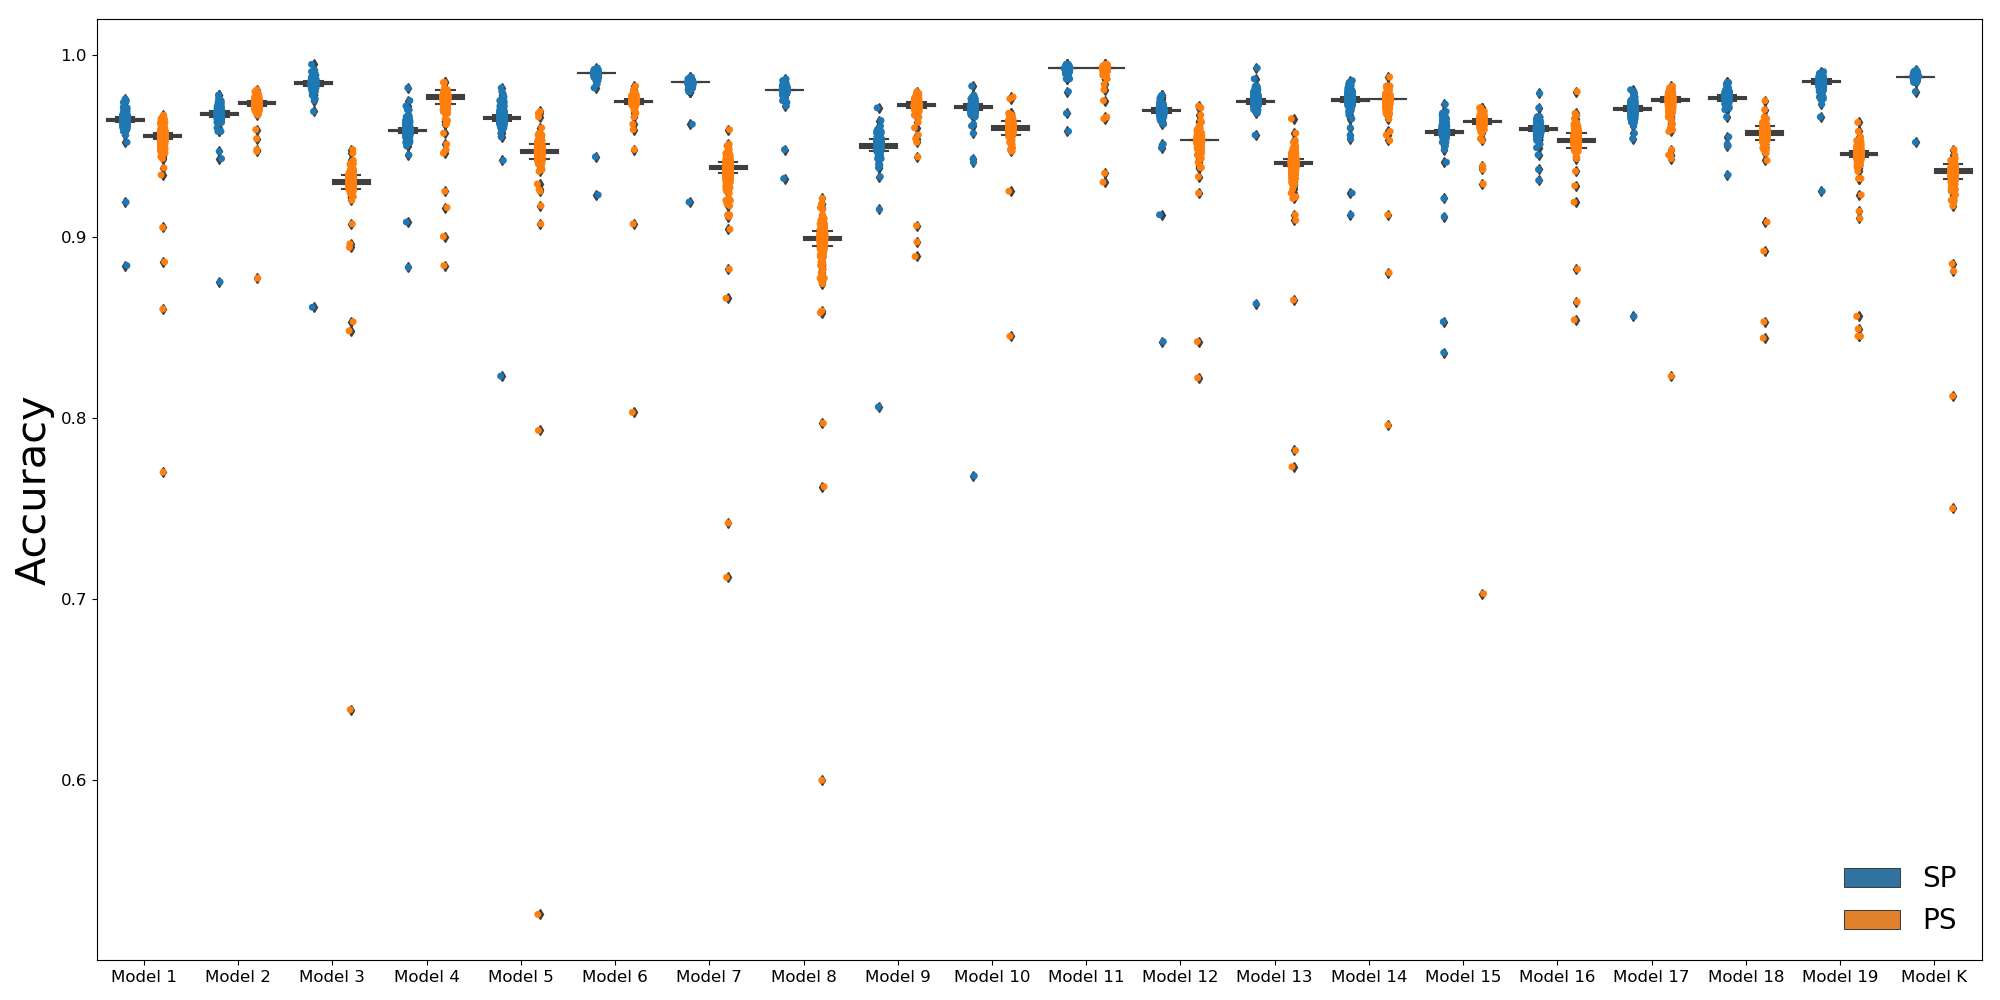
\includegraphics[width=15cm]{figures/Ablation_results_all_models.png}
    \caption{\textbf{Ablation results for all 20 models}}
    \label{fig:ablation_all_models}
\end{figure*}


\begin{figure*}
    \centering
    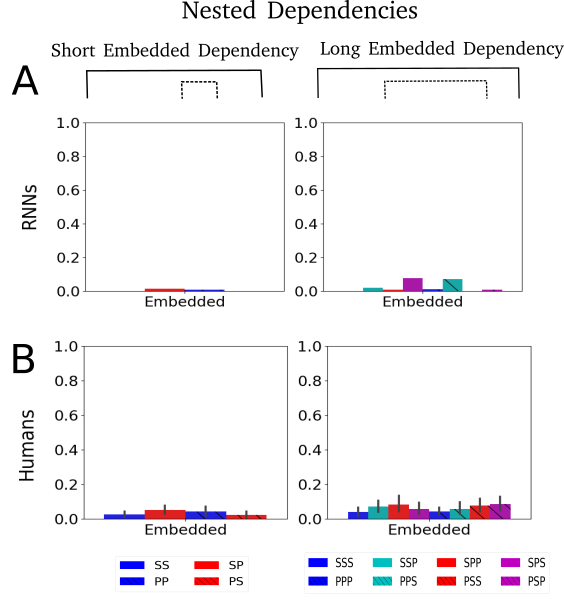
\includegraphics[width=10cm]{figures/error_rates_successive_all_conditions.png}
    \caption{\textbf{Error rates on Short- and Long-Successive:} collected from NLMs (panel A) and human subjects (B). Blue and red colors correspond to congruent and incongruent subjects, respectively. Secondary colors (cyan and magenta) indicate an attractor with an opposite number. Slant lines in bars indicate that the main subject is plural.}
    \label{fig:successive_all_conditions}
\end{figure*}
    
    
\begin{figure*}
    \centering
    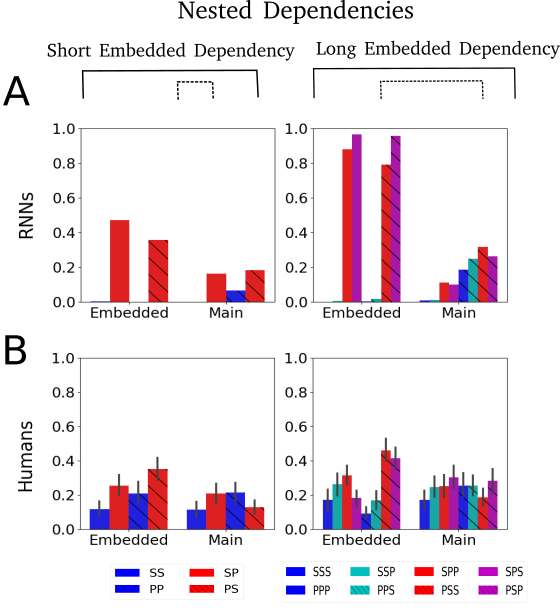
\includegraphics[width=10cm]{figures/error_rates_nested_all_conditions.png}
    \caption{\textbf{Error rates on Short- and Long-Nested:} collected from NLMs (panel A) and human subjects (B). Blue and red colors correspond to congruent and incongruent subjects, respectively. Secondary colors (cyan and magenta) indicate an attractor with an opposite number. Slant lines in bars indicate that the main subject is plural.}
    \label{fig:nested_all_conditions}
\end{figure*}
    
    


\end{document}